% =============================================================================
\section{Choice of grid}
\label{sec:bec-noise:grid}
% =============================================================================

In the previous section we mentioned that the spatial grid size for interferometry simulations was chosen to be $8\times8\times64$.
This is the point of equilibrium for two conflicting requirements.
First, the number of grid points (which corresponds to the number of modes) must be low enough to satisfy the Wigner truncation condition~\eqnref{wigner-bec:truncation:population-condition}.
Second, the number of grid points must be high enough to describe the dynamics of the condensate.

The grid
\begin{eqn}
    \mathbf{G}_{\mathrm{ref}}
    \equiv G_{\mathrm{ref}}^x \times G_{\mathrm{ref}}^y \times G_{\mathrm{ref}}^z
    = 8\times8\times64
\end{eqn}
grid was picked as the starting point for several reasons:
\begin{itemize}
\item it has $4096$ points, which is about an order of magnitude lower than the target population $N=55,000$;
\item its shape corresponds to the shape of the trap (in other words, the spacings in every direction are close to each other);
\item the number of points in each dimension is a power of $2$, which is convenient for numerical calculations.
\end{itemize}
The box for this grid was set to be $1.2$ times wider in all directions than the Thomas-Fermi ground state~\eqnref{bec-noise:mean-field:tf-gs} for the target population.
This resulted in the box
\begin{eqn}
    \mathbf{B}_{\mathrm{ref}}
    \equiv B_{\mathrm{ref}}^x \times B_{\mathrm{ref}}^y \times B_{\mathrm{ref}}^z
    = 9.10\un{\mu m}\times8.83\un{\mu m}\times75.48\un{\mu m},
\end{eqn}
which was used as the reference point.

The test consisted of running the simulation for the Ramsey sequence with the time $t=1.3\un{s}$ and comparing resulting vectors $\mathbfcal{V}$, consisting of $100$ sampled values of $\mathcal{V}(t)$ for times from $0\un{s}$ to $1.3\un{s}$, as
\begin{eqn}
    \Delta \mathcal{V}_{\mathrm{grid, box}}
    =
        \left\|
            \mathbfcal{V}_{\mathrm{grid, box}}
            - \mathbfcal{V}_{G_{\mathrm{ref}}, B_{\mathrm{ref}}}
        \right\|_2 /
        \left\|
            \mathbfcal{V}_{G_{\mathrm{ref}}, B_{\mathrm{ref}}}
        \right\|_2.
\end{eqn}

In different runs we varied axial and radial grid spacing (box length divided by the number of points in the corresponding dimension) separately.
Since the integrating algorithm performed best with numbers of grid points being powers of $2$, the required spacing was achieved by changing both box length and grid size (for example, the axial spacing $0.75$ of the reference one was achieved by using $2 G_{\mathrm{ref}}^z$ grid points in the $z$ direction, and $1.5 B_{\mathrm{ref}}^z$ box size in that direction).
To check this approach we ran two additional tests with doubled box length and grid points number in both directions separately, which resulted in additional points for relative spacing $1.0$ in \figref{bec-noise:grid:spatial-convergence}.
They are very close to the reference points (which have $y$-coordinate equal to zero), which proves that the $\Delta \mathcal{V}$ value is only sensitive to the grid spacing and not to the box or grid sizes separately.

\begin{figure}
    \centerline{%
    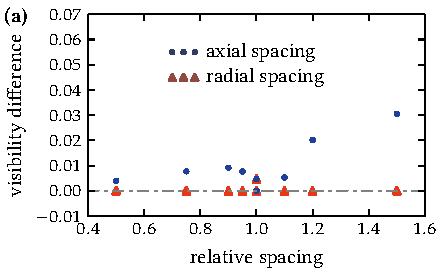
\includegraphics{figures_generated/test/grid_check_gpe.pdf}%
    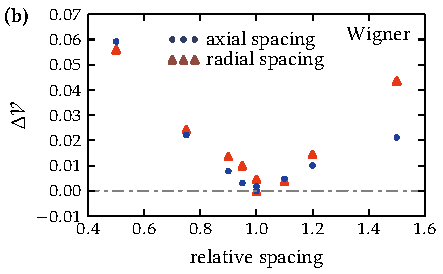
\includegraphics{figures_generated/test/grid_check_wigner.pdf}}

    \caption[Spatial convergence test]{
    Spatial convergence test.
    }%endcaption

    \label{fig:bec-noise:grid:spatial-convergence}
\end{figure}

In order to check only the effect of spatial resolution without being influenced by changing number of modes, we performed a batch of tests for \abbrev{cgpe}s~\eqnref{bec-noise:mean-field:cgpes-simplified} in addition to the truncated Wigner \abbrev{sde}s~\eqnref{bec-noise:wigner:sde}.
The results for \abbrev{cgpe}s are plotted in \figref{bec-noise:grid:spatial-convergence},~(a).
It is evident that further decrease of spacing both in radial and axial directions does not change the results much.
On the other hand, when the axial spacing is increased, $\Delta \mathcal{V}$ starts to grow.
This means that the reference grid $G_{\mathrm{ref}}$ has enough spatial resolution for our purposes.

For the truncated Wigner \abbrev{sde}s, \figref{bec-noise:grid:spatial-convergence},~(b) shows that the decrease of radial or axial spacing as compared to reference values still changes the results significantly.
But since it is not observed in \abbrev{cgpe}s case, we must conclude that this is the result of the criterion~\eqnref{wigner-bec:truncation:population-condition} being violated.
Even at $t=0\un{s}$ the number of modes for the reference grid is only ten times smaller than $N=55,000$, and at $t=1.3\un{s}$ the population becomes $2$ times smaller due to losses (see \figref{bec-noise:visibility:echo-visibility},~(a))
Therefore, the further increase of the number of grid points and, therefore, modes, makes the truncated Wigner results unreliable.

In view of the tests in this section, we have chosen the grid $\mathbf{G}_{\mathrm{ref}}$ and the box $\mathbf{B}_{\mathrm{ref}}$ for all the interferometry simulations.

It must be noted that it is possible to decouple the grid size and the number of modes by applying the projector in~\eqnref{bec-noise:wigner:sde} explicitly instead of relying on the implicit cutoff enforced by the grid.
This requires grid padding to avoid aliasing~\cite{Norrie2006}, and thus significantly increases simulation time.
On the other hand it does not give much in terms of spatial resolution, since, with higher frequency modes being projected out in mode space, the corresponding fine details in the coordinate space disappear.
Therefore in this thesis we have settled with using only implicit cutoff.
